% \documentclass[article,reqno]{amsproc}
% \documentclass[twocolumns,aps,rmp]{revtex4-2}
\documentclass[aps,rmp,twocolumn,nofootinbib,superscriptaddress,floatfix,longbibliography]{revtex4-2}
\usepackage{amsmath,amssymb, mathtools}
% \usepackage[,es-tabla]{babel}
\usepackage{graphicx}
\usepackage{caption}
\usepackage{bm,lipsum}
\usepackage{cancel}
\usepackage{textcomp}
\usepackage{enumitem}
\usepackage{gensymb}
\usepackage{empheq}
\usepackage{siunitx}
\usepackage{physics}
\usepackage{bbold}
% \usepackage[a4paper]{geometry}
% \geometry{top=1.5cm, bottom=1.2cm, left=2.2cm, right=2.2cm}
\setlist{noitemsep,leftmargin=*}
\newcommand*\widefbox[1]{\fbox{\hspace{2em}#1\hspace{2em}}}
\newcommand{\powerset}{\raisebox{.15\baselineskip}{\Large\ensuremath{\wp}}}
\usepackage{hyperref}
\hypersetup{
colorlinks=true,
urlcolor= blue,
citecolor=blue,
linkcolor= blue,
bookmarks=true,
bookmarksopen=false,
}


\setcitestyle{square}

% \makeatletter
% \g@addto@macro{\CTEX@section@format}{\raggedright}
% \makeatother

% \numberwithin{equation}{section}
\usepackage{caption}
\usepackage{fancyhdr}
\usepackage{braket}
\pagestyle{fancy}
\lhead{Técnicas Observacionales 2024-I}
\begin{document}

\title{\large Street lights as standard candles: an example in National University of Colombia campus }

\begin{abstract}
\normalsize
\begin{center}\textbf{Abstract}\\
\end{center}
This activity was developed to showcase one of the processes involved in astronomical measurements. Standard candles are used as cosmic lighthouses to determine the distance to far objects \cite{paper_possel}. For showcasing the method astronomers use, we used a group of lined-up street lights on UNAL campus, and measured their brightness using SAOImage software, to then use the inverse square law, to obtain the distances to each of these lights. We found an overall low relative error to the real measured distances, although a couple lights had trouble. To deal with the outliers we performed a comparative analysis between the decrease of the brightness of the streetlight and that of a type IA supernova, which is given by their corresponding light curves (more precisely the time after a peak luminosity).
 
\textbf{Keywords:} Standard candles, Astronomical measurements, intrinsic brightness, light curve.
\end{abstract}


\author{Eduardo A. Delgadillo M. }
\affiliation{Observatorio Astronómico Nacional, Universidad Nacional de Colombia, Bogotá, Colombia}

\author{Edwin C. Laverde V.}
\affiliation{Departamento de Física, Universidad Nacional de Colombia, Bogotá, Colombia}


\rhead[]{\today}

\maketitle
\thispagestyle{fancy}


\section{Introduction}
For many years, determining distances beyond our solar system was the primary challenge. It was extremely difficult to discern which objects in the sky belonged to our stellar neighborhood. 
In standard candles, astronomers found an efficient and certain method to resolve object distance. It is assumed that some objects possess an unvarying, constant, and intrinsic brightness. If this proves to be true, it would mean that it could be possible to establish a relationship between apparent brightness and distance. This relationship is known as the inverse square law.

\section{Theoretical Framework}

Possibly the most important variable in astrophysics is distance. But to measure distance to objects that are incredibly far away, using regular methods is not feasible in any way. Thus it could be really useful for an astronomer to be able to know the distance to an astrophysical object using other properties of such object that they can measure properly. One such case is that of the luminosity of an object. Assuming  that the object's emission is isotropic, and considering the fact that the apparent brightness of the object as seen by an observer at a distance $d$ follows an inverse-square law, it can be shown that the flux at the observer is related to the luminosity of the object and the distance at which it is seen as follows:
\begin{equation}
    F = \frac{L}{4 \pi d^2}
    \label{flux}
\end{equation}
Having this equation, one could solve for the distance, measure the flux, and given the object has a known luminosity, find how far away the object is.

The objects whose intrinsic brightness is known are called \textit{standard candles}, some examples are Cepheid variables and Type IA supernovae.

To demonstrate the method astronomers use for measuring astronomical distances we will use street lights as our mock standard candles. For this, we assume these street lights have an intrinsic common brightness, which in this case is not readily available. Although we don't a priori know the value of $L$ from equation \eqref{flux}, we can take a given street light (say the closest), and establish its calculated luminosity (through equation \eqref{flux}), and use this value in equation \eqref{flux} for all the other street lights. This means that the master equation we'll use for calculating the distance to a given street light $i$ is:
\begin{equation}
    d_i = d_0 \sqrt{\frac{F_0}{F_i}}
    \label{dist}
\end{equation}


\section{Analysis and Results}
For the demonstration of the application of the inverse square law and the standard candles method, a street at the National University of Colombia was selected. This street has a large number of streetlights, is a linear avenue, and does not have many obstacles. 
Using a digital camera the line of lights can be captured in a single image. The digital camera used is a Nikon D5600. A picture of the streetlights along the long road was captured, the image taken is shown in Fig. \ref{fig:1}. An important remark to make now is the fact that the 8th street light is actually turned off, so we will take that into account in the following analysis.
\begin{figure}
    \centering
    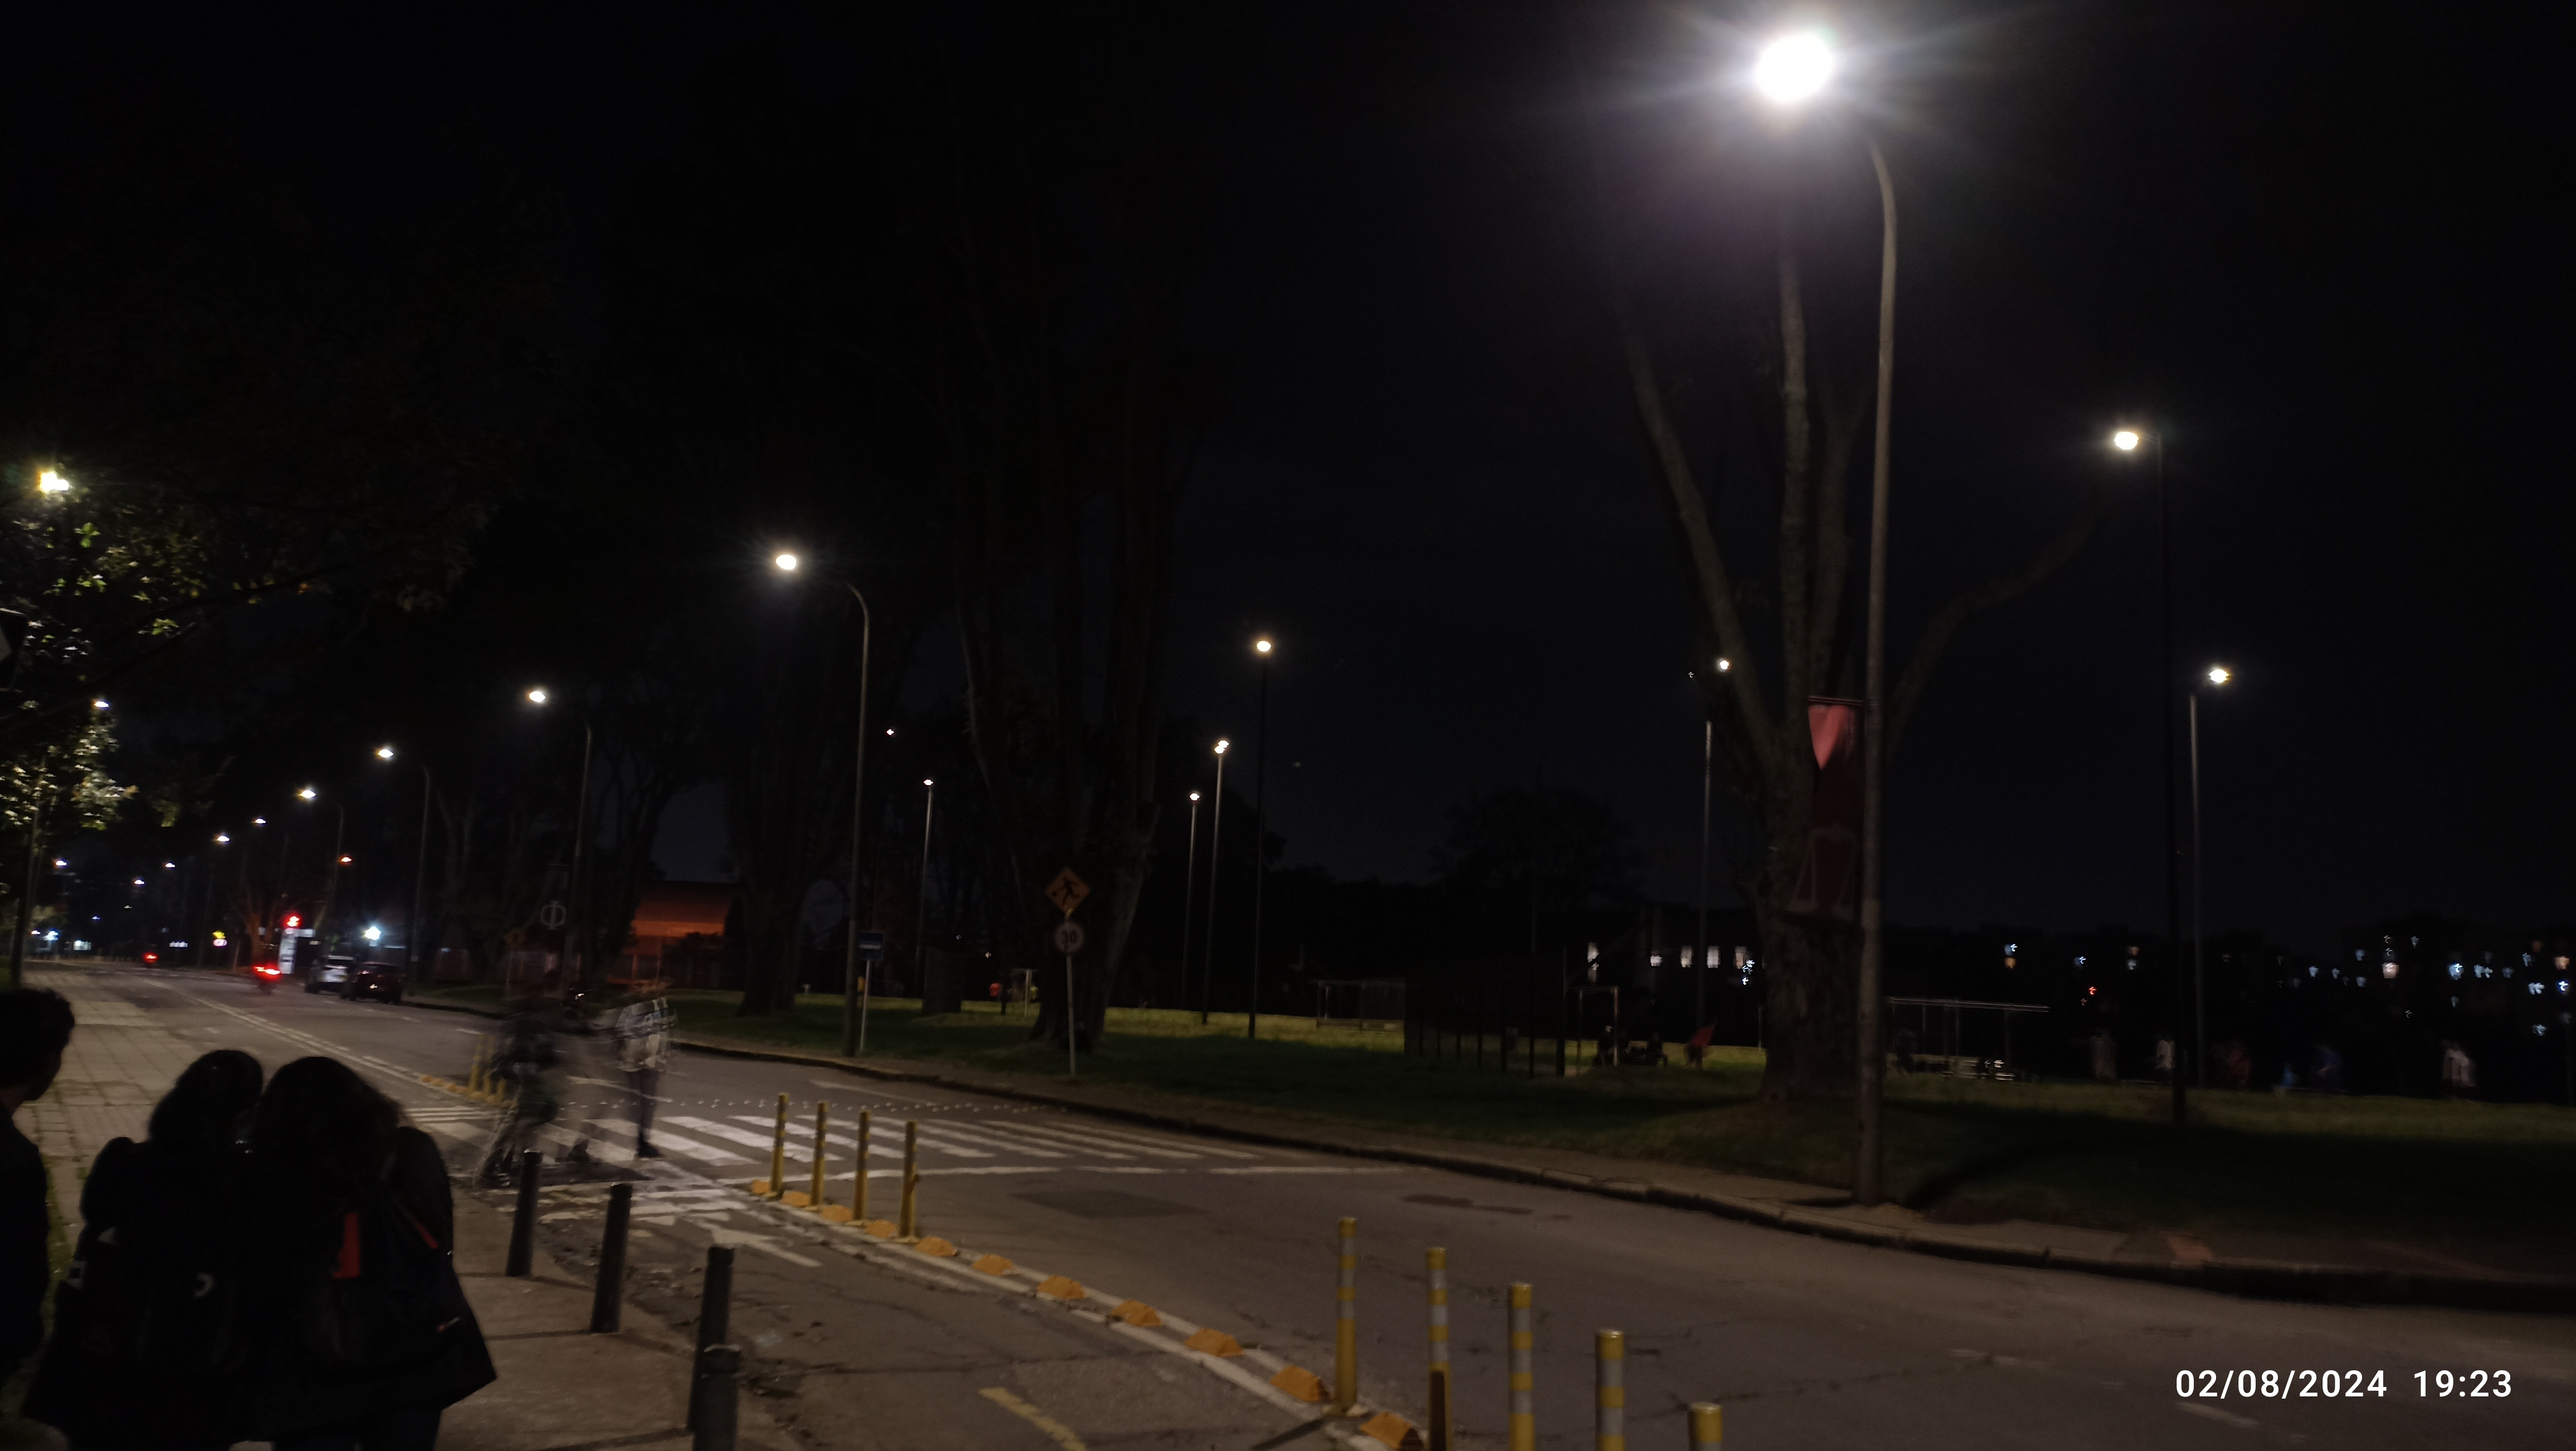
\includegraphics[width=0.47\textwidth]{Images/DSC_1347.jpg}
    \caption{Image of site.}
    \label{fig:1}
\end{figure}

It was necessary to adjust some photographic parameters in the digital camera to obtain an image with the lights shining through. The focal aperture was defined  in f/9.0 and the shutters speed in 1/4000 sec. The image obtained is shown in figure \ref{fig:2}. It's worth noting this image is cropped as not to show the first, brightest, light that can be seen in the previous image. This is due to the fact that we won't be using this first light since some of it's pixels were saturated.

\begin{figure}
    \centering
    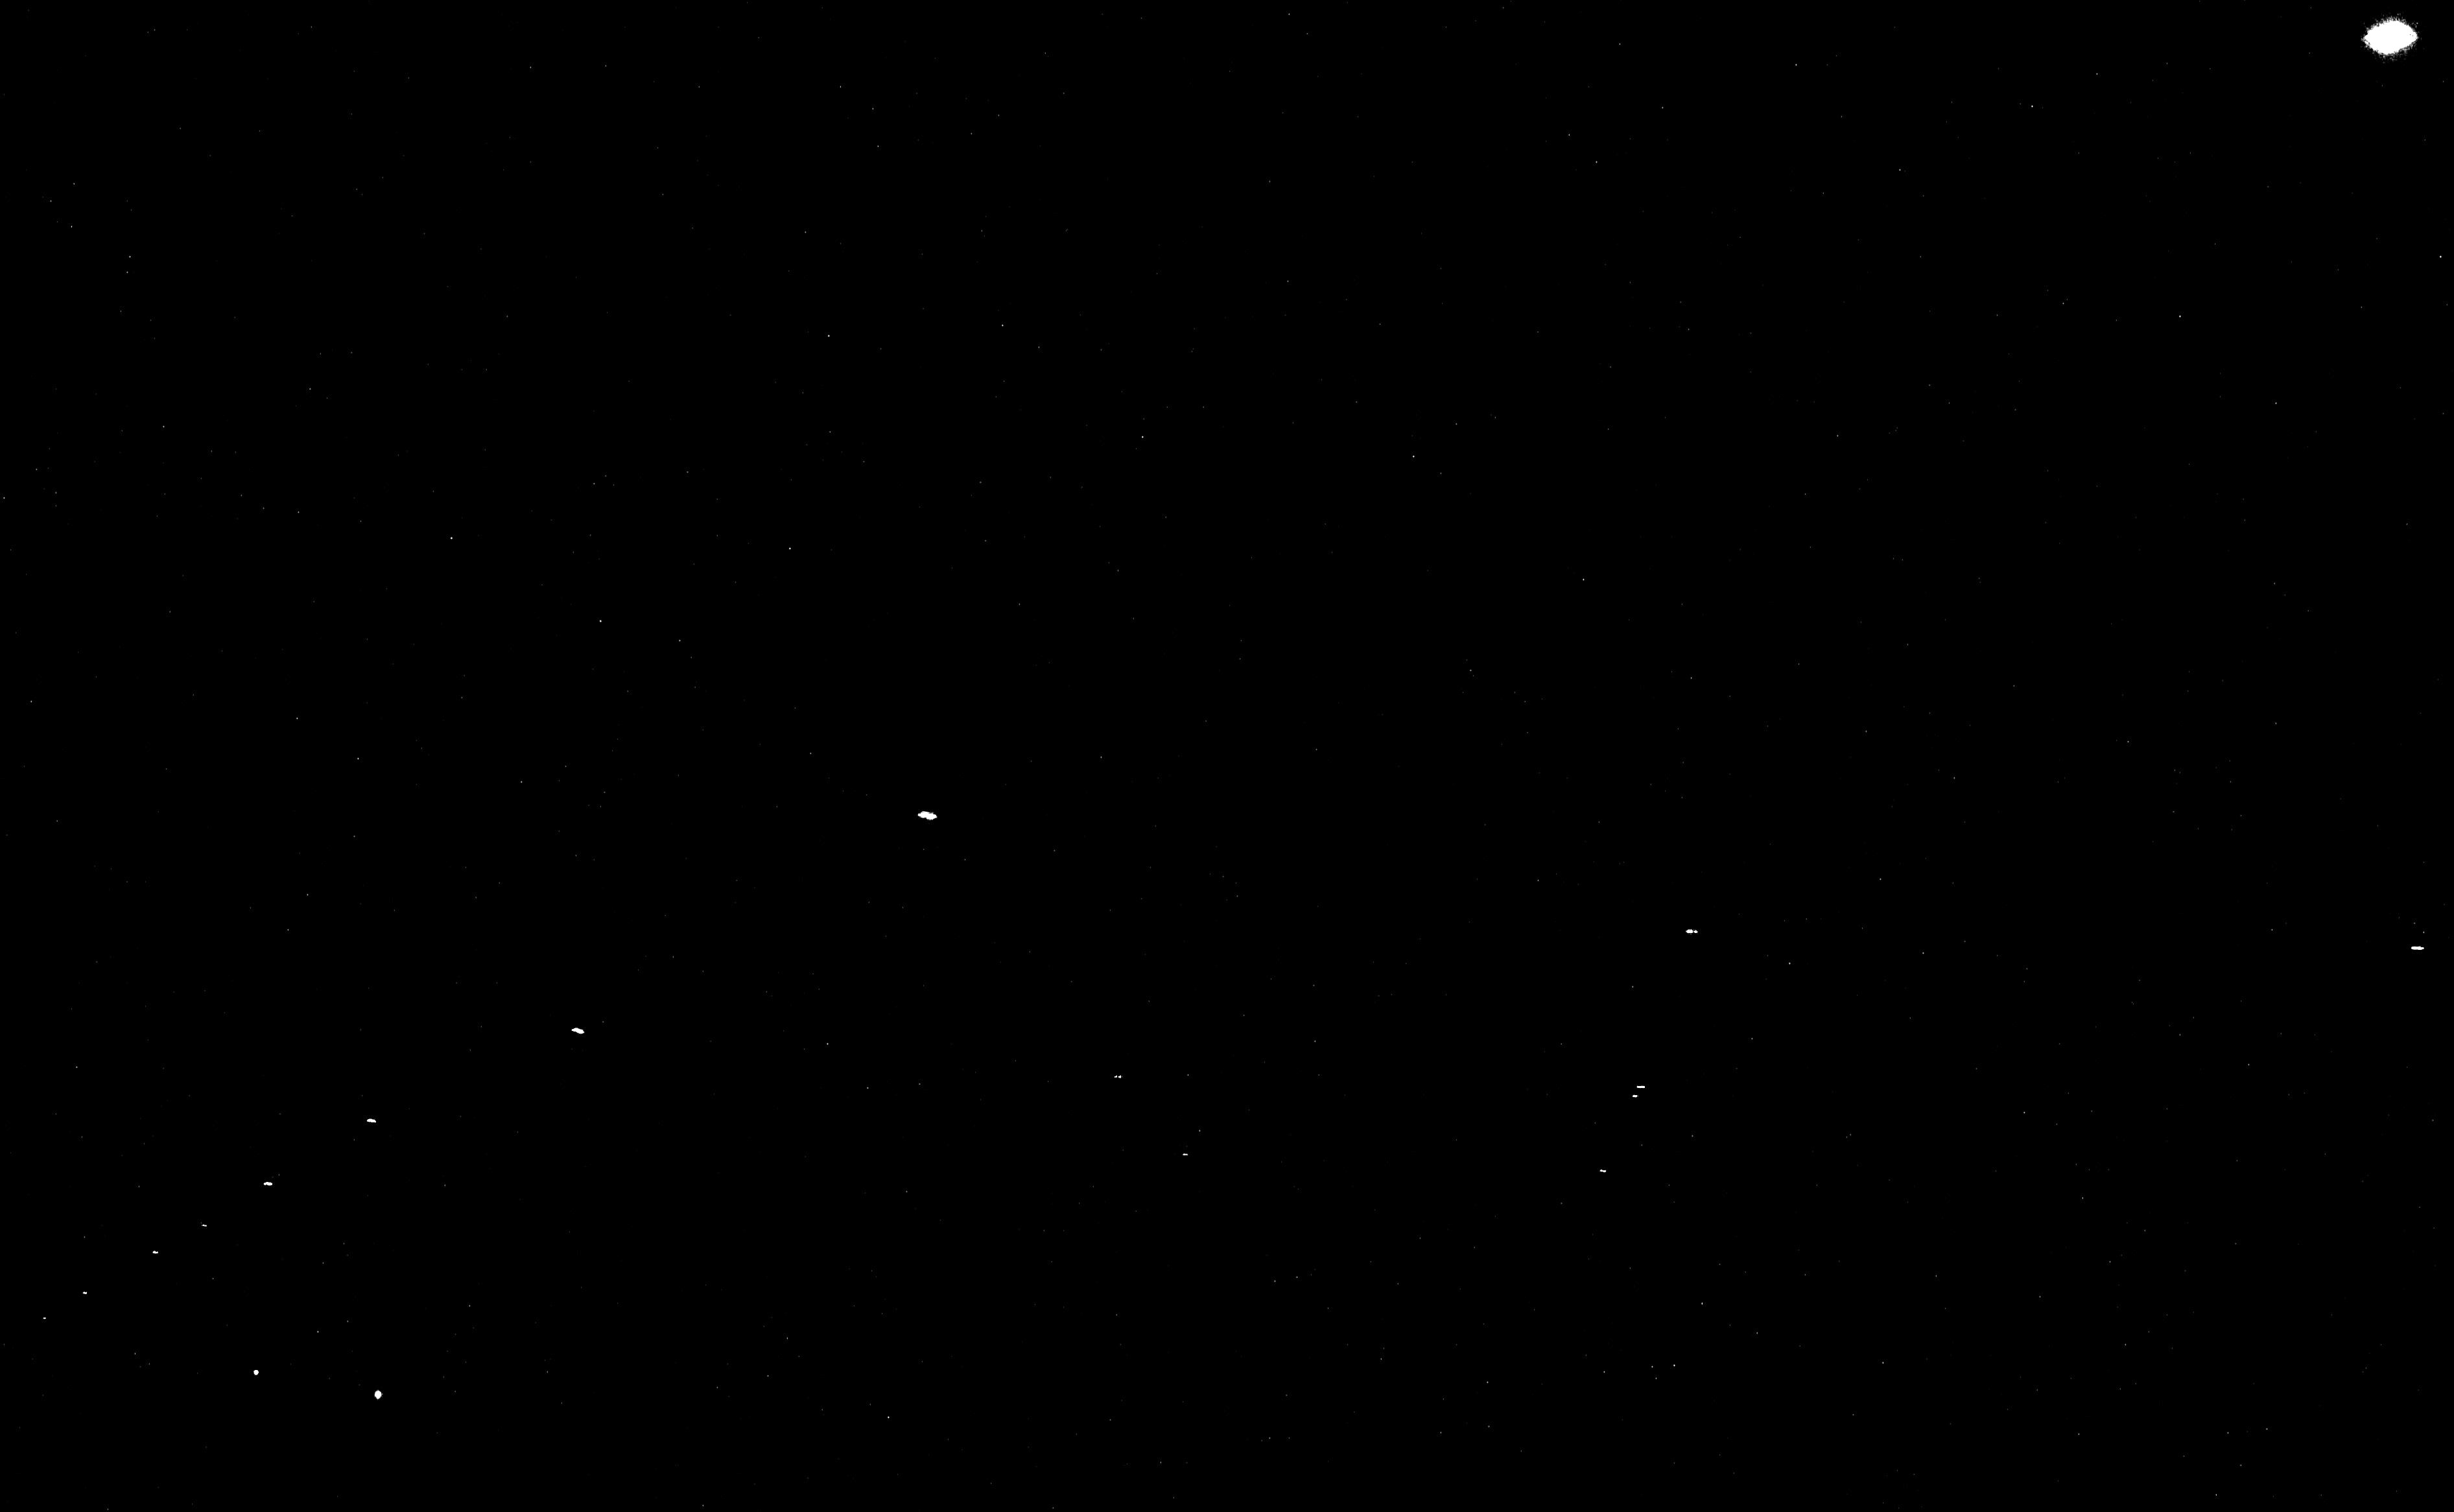
\includegraphics[width=0.47\textwidth]{Images/DSC_1347_.jpeg}
    \caption{Image after adjusting camera parameters. The line of street lights can clearly be seen.}
    \label{fig:2}
\end{figure}

Once the image was taken, it was processed using \textit{SAOimageDS9} software to remove noise and exclude unwanted objects. By using an ellipse-shaped region, which was overlaid on the different lights, we obtained the pixel values sum, mean, and median. To remove possible background noise from this data, we obtained the same data corresponding to a smaller similarly-shaped region near the light and then substracted these values from the ones of the light. One of the regions used can be seen in Fig. \ref{fig: ellipse}.
\begin{figure}[h]
    \centering
    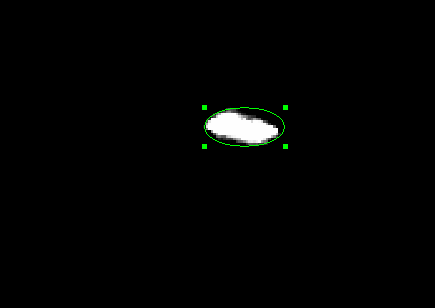
\includegraphics[width=0.41\textwidth]{Images/Ellipse_region.png}
    \caption{Ellipse-shaped region used for obtaining pixel data from the street lights.}
    \label{fig: ellipse}
\end{figure}

Following this simple procedure for all the lights, we obtain the information we need. However, to find the distances using equation \eqref{dist}, we need to multiply the obtained pixel values by the area of the regions we used (for both the lamp and background regions). Doing this, we can graph the expected measured distances, along with the distances obtained using this method. This can be seen in the upper part of Fig. \ref{fig: Mean0}. The lower part shows the relative difference between these values. It is immediatly clear that something is off. The error of the first 3 lights is relatively large, and that of the next ones is even larger.

To explain this, we have to take a look at the regions we chose for enclosing the street lights (Fig. \ref{fig: ellipse}). It is clear that this region is enclosing other pixels which do not belong to the light of interest, namely background pixels. As such, given their dark appearance, this pixels have rather low values. As is known, the mean of a distribution is easily affected by outliers (extreme values), and since there are quite a few background pixels, which are certainly not anywhere near the mean values of the light-only pixels, they are definitely bringing the mean down from it's real value. This way, the discrepancy seen in Fig. \ref{fig: Mean0} can be traced back to the choice of the mean to find the flux.
\begin{figure}[h]
    \centering
    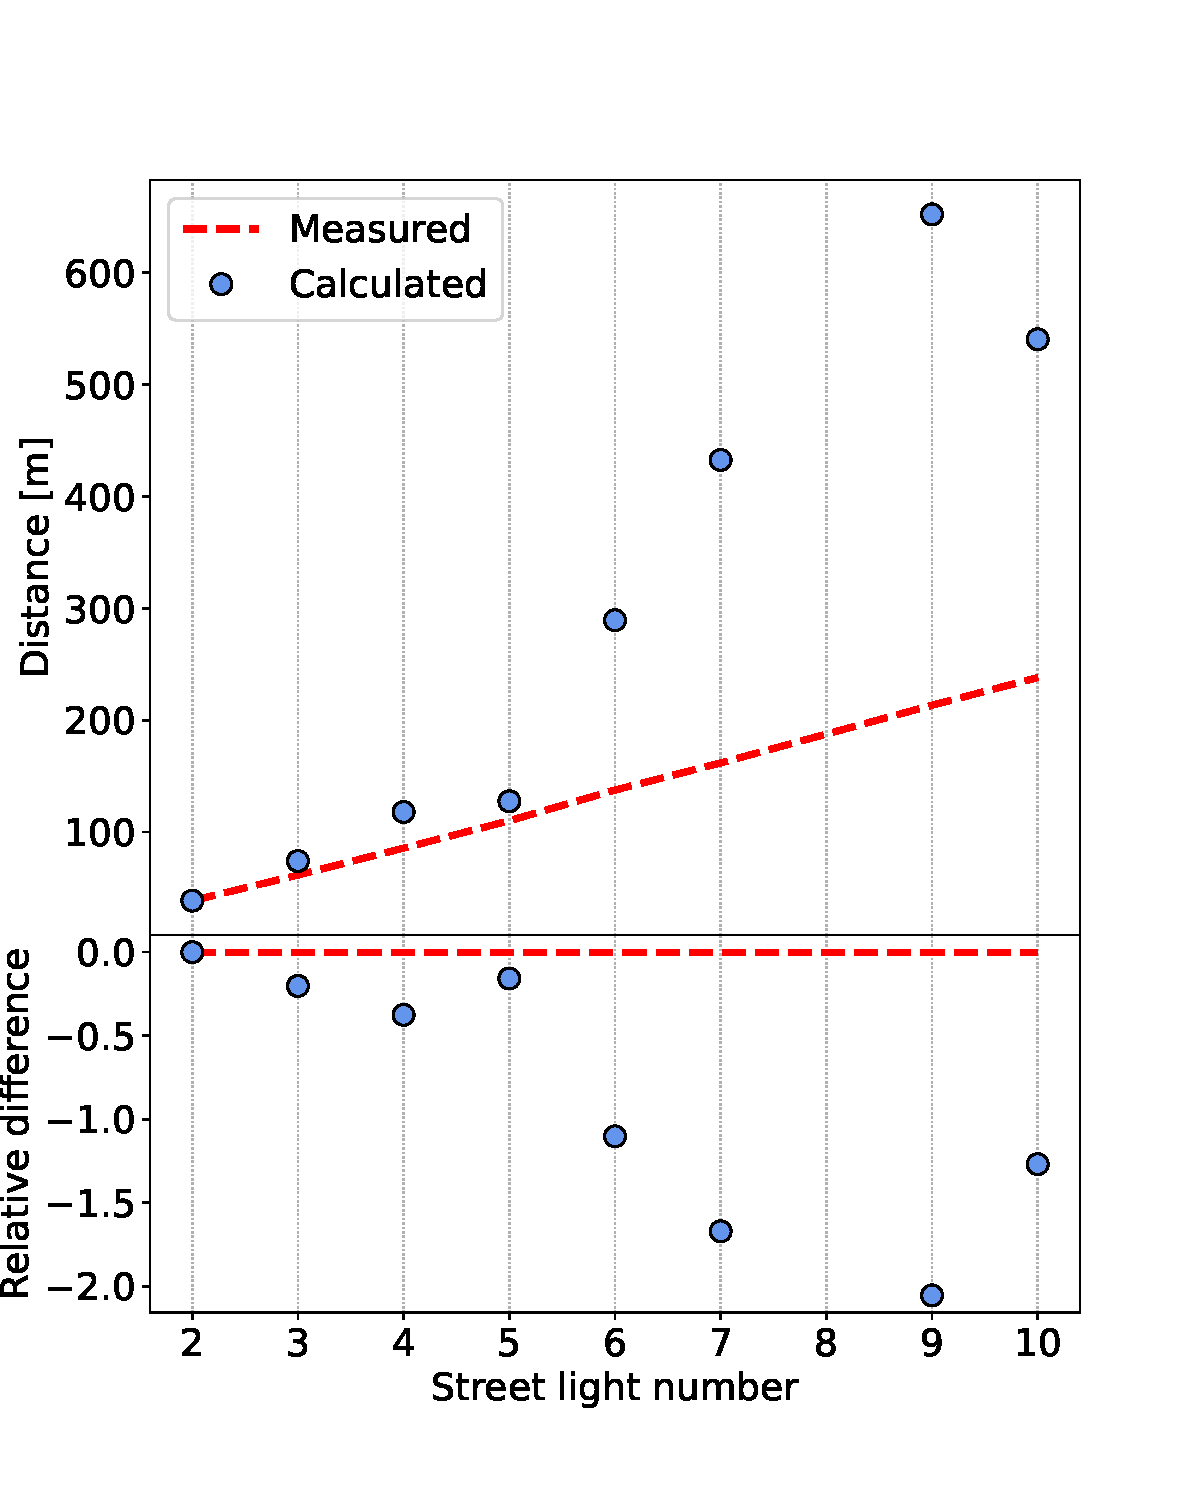
\includegraphics[width=0.5\textwidth]{Images/PlotMean.pdf}
    \caption{Top: Distances to street lights calculated with the mean pixel value inside elliptical regions, and expected (measured) distances. Bottom: Relative difference between found and measured distances.}
    \label{fig: Mean0}
\end{figure}

To fix the discrepancy, we change the ellipse-shaped region for a new polygon region, which allows us to better enclose the light, making the results more reliable. We also turn to using the median of the pixels inside the region since the median is a quantity that is less affected by outliers. Using this new data, we obtain what's shown in Fig. \ref{fig: Median0}.
\begin{figure}[h]
    \centering
    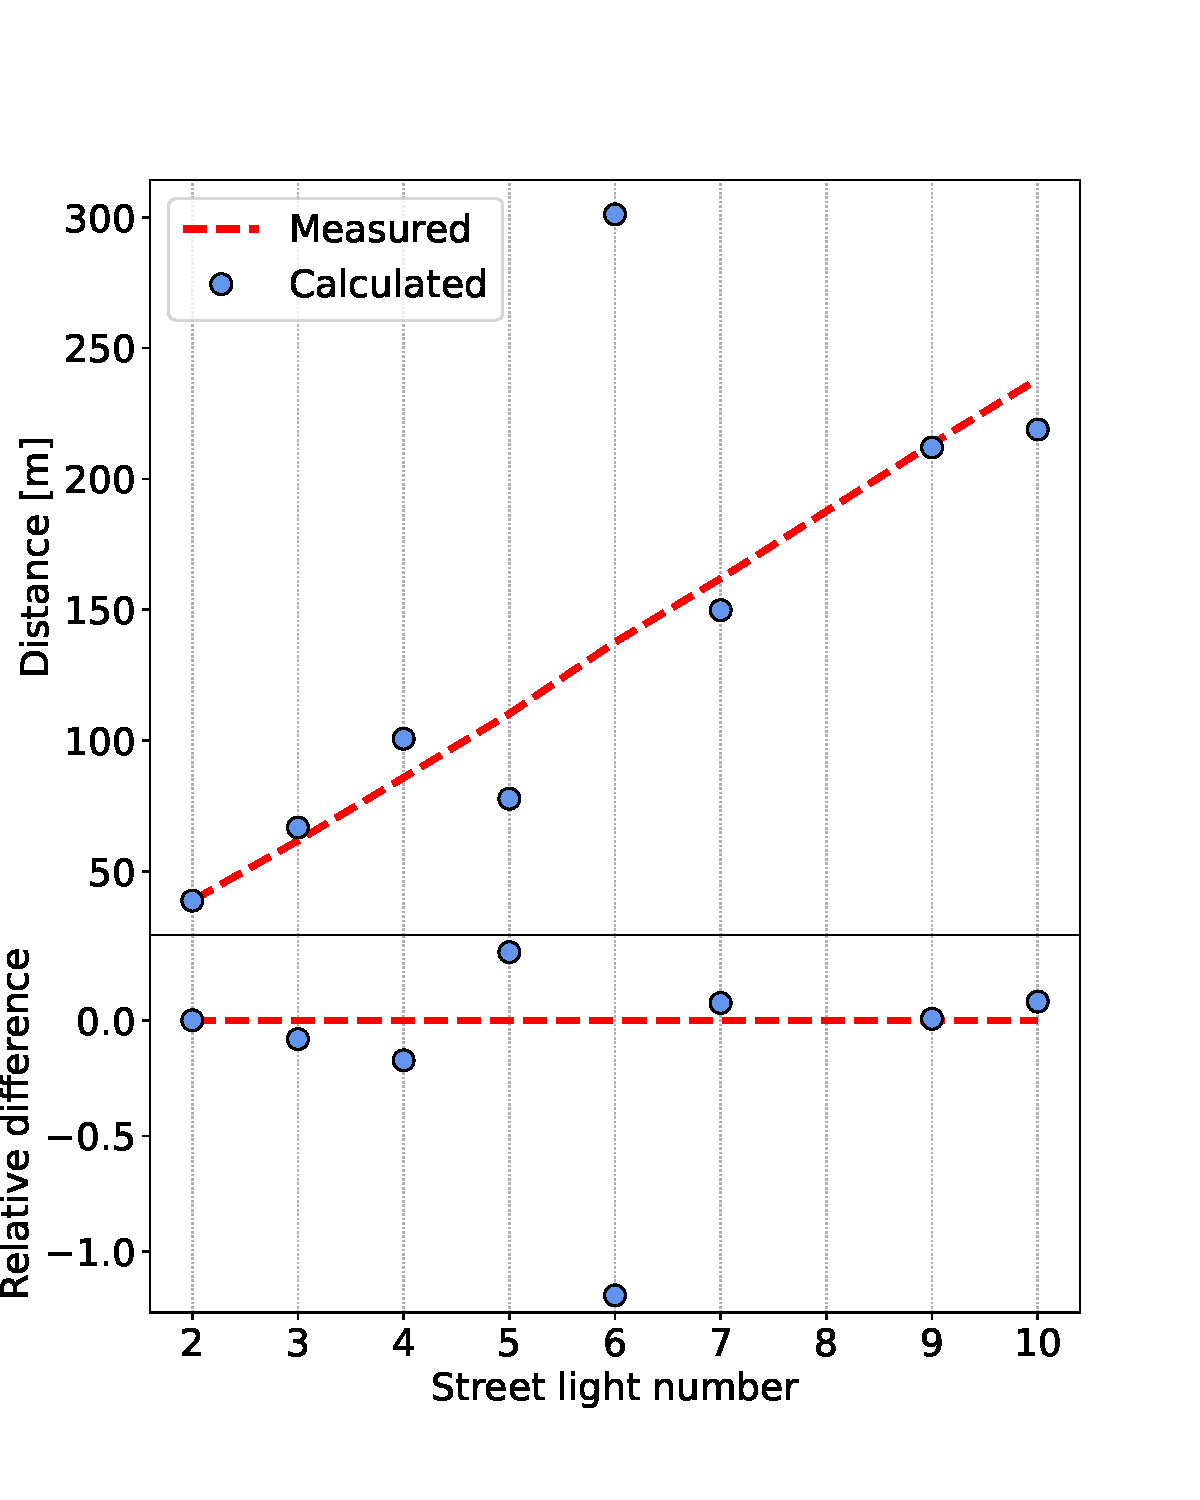
\includegraphics[width=0.5\textwidth]{Images/PlotMedian.pdf}
    \caption{Top: Distances to street lights calculated with the median pixel value inside elliptical regions, and expected (measured) distances. Bottom: Relative difference between found and measured distances.}
    \label{fig: Median0}
\end{figure}

A considerable improvement can already be observed. Most of the points are now closer to the expected behaviour, and their errors are relatively smaller. However, it is also clear that there's still a point that is not quite following the overall tendency (outlier), that is street light number 6. Let's first look at it on the original picture. A zoomed-in version of this image is shown in Fig. \ref{fig: zoom6}. Visually it can easily be seen that street light number 6 is certainly dimmer than the surrounding lights, even dimmer than ones that are farther away. This indicate an intrinsic problem with this light, its luminosity is not equal, or even considerably near, that of the other lights.
\begin{figure}[h]
    \centering
    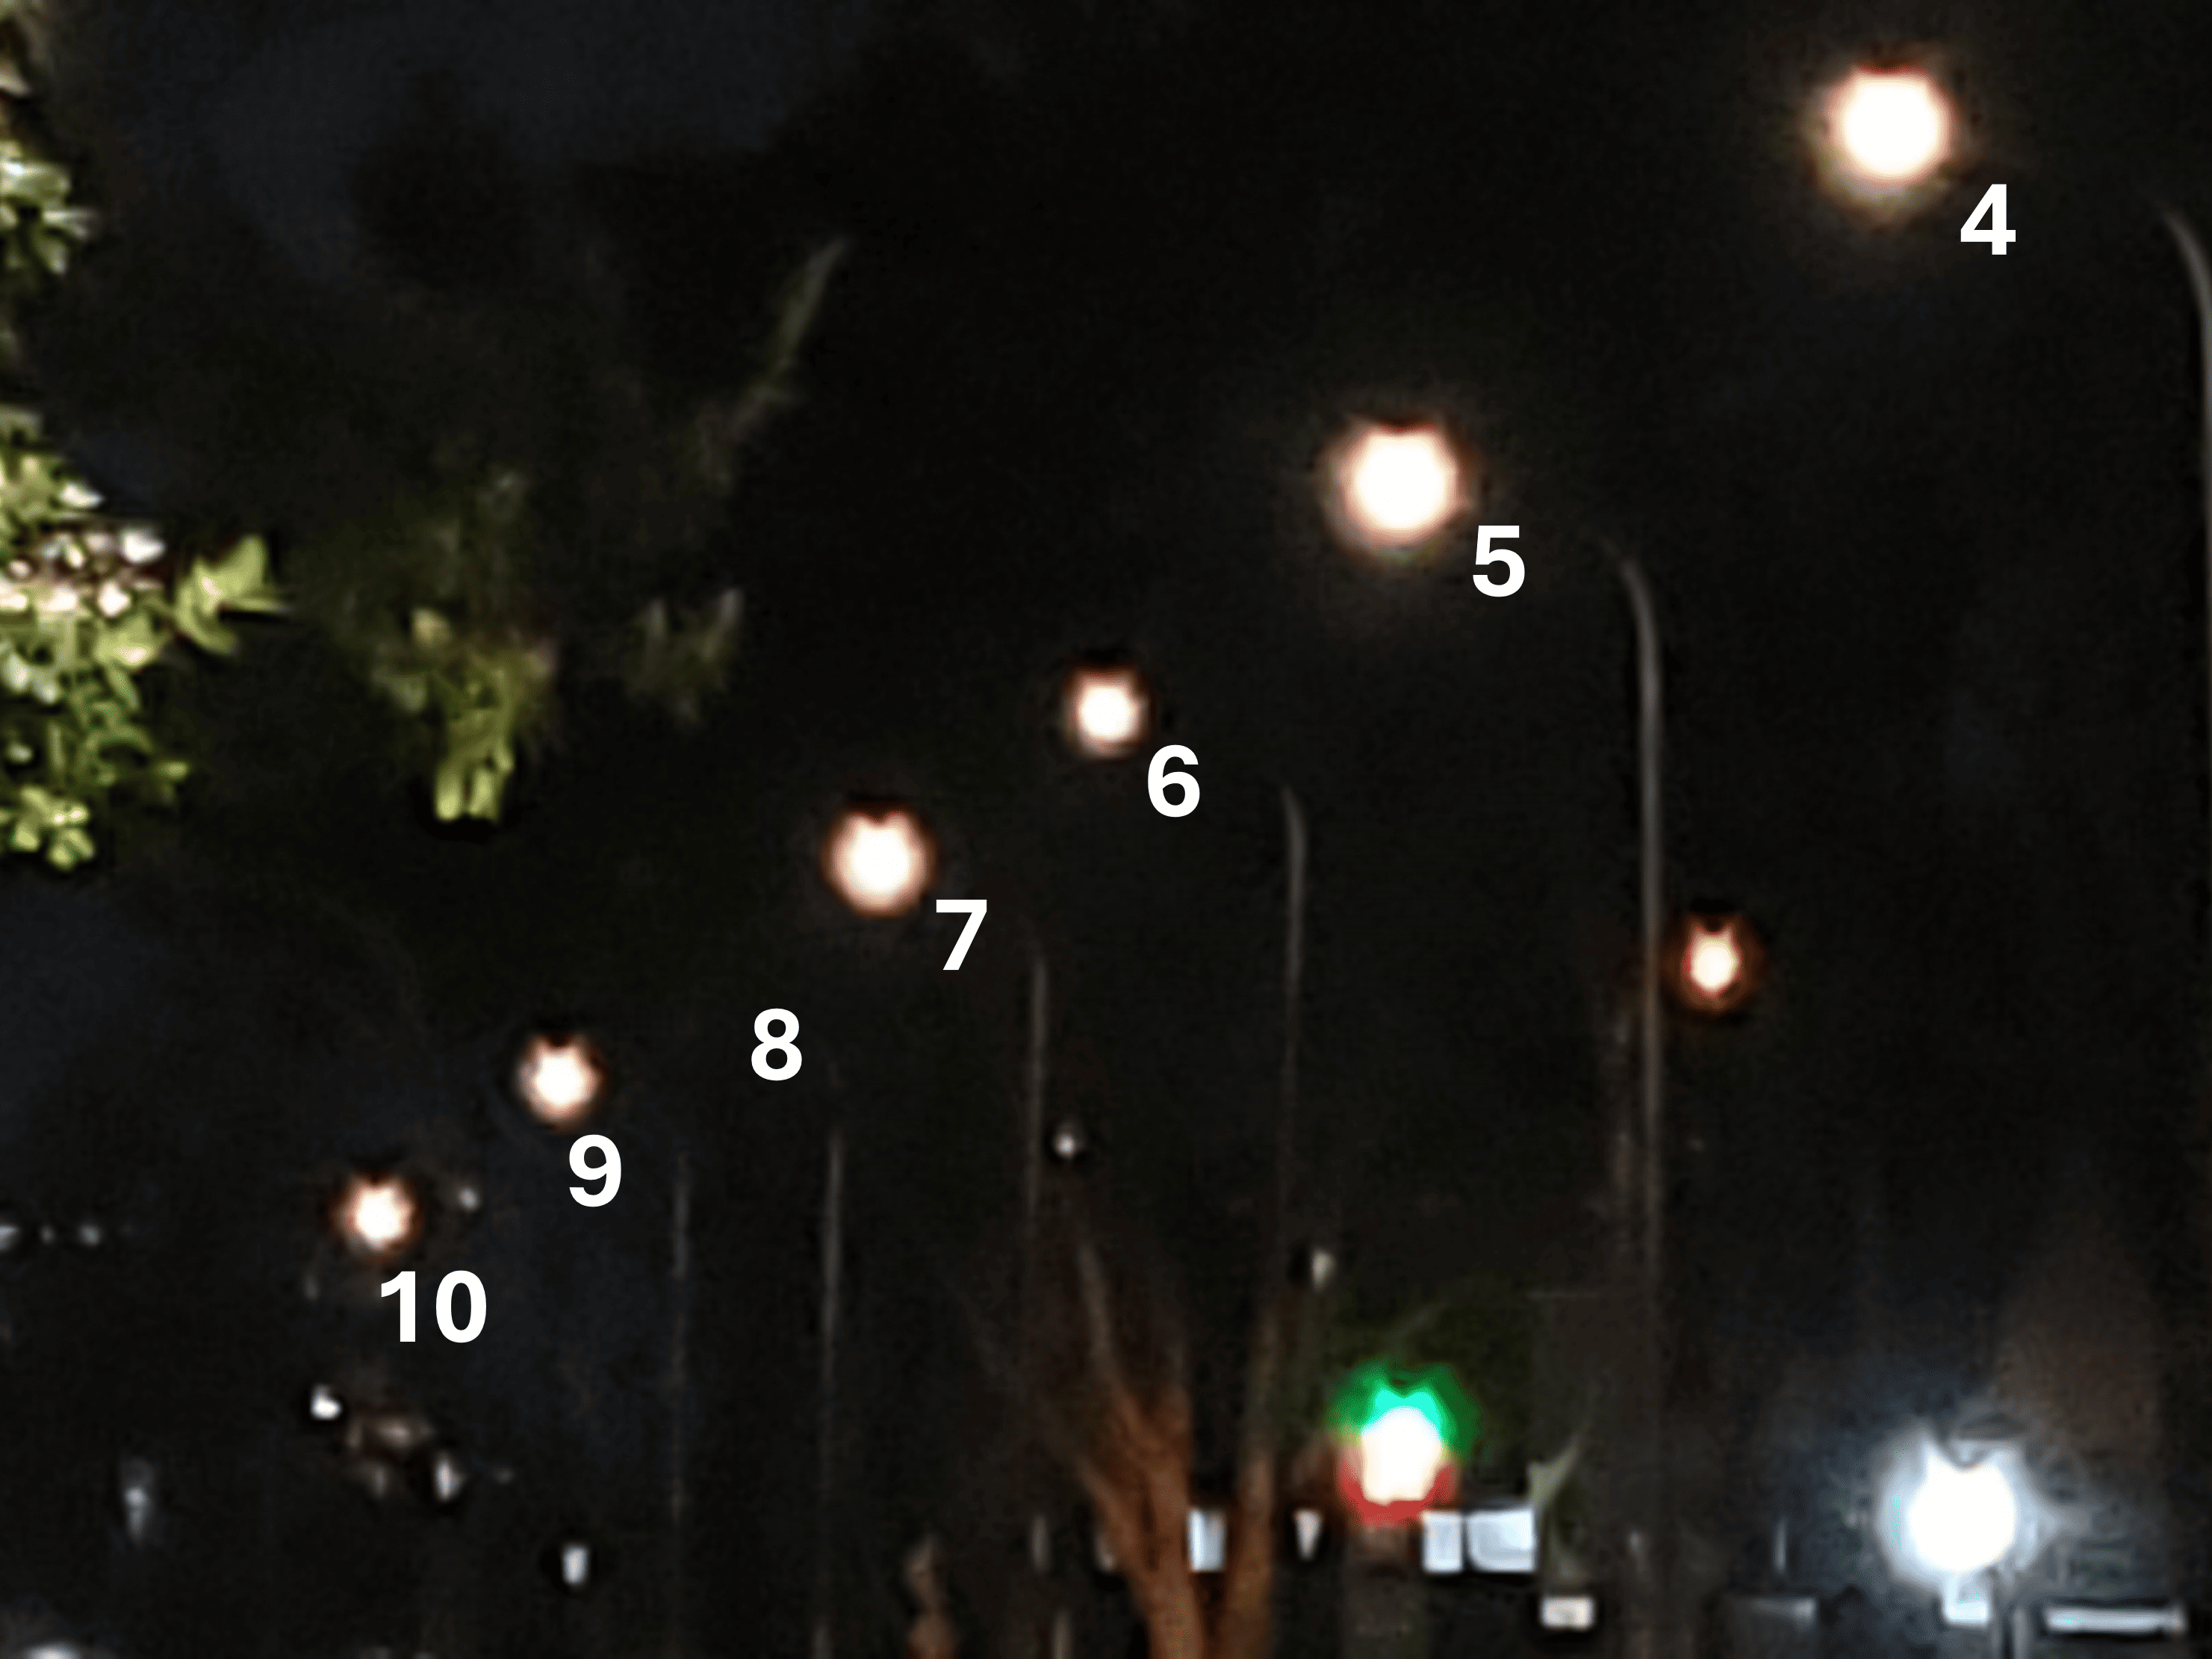
\includegraphics[width=0.4\textwidth]{Images/zoom6.png}
    \caption{Original image zoomed-in in the vicinity of light 6.}
    \label{fig: zoom6}
\end{figure}


To deal with this, we use the most famous distance indicators: type IA supernovae. These standard candles are used due to their known characteristic brightness with approximately constant luminosity. There exists a correlation between the time scale of the explosion and its peak luminosity. The intensity of luminosity decreases with the passing days of light and is represented in a light curve at peak luminosity. For illustration, a theoretical chart is showed in
Fig. \ref{fig: Supernovae}.
\begin{figure}[h]
    \centering
    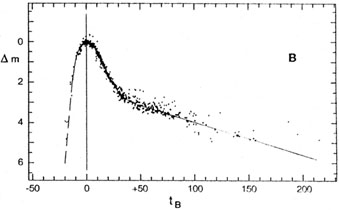
\includegraphics[width=0.5\textwidth]{Images/Supernovae.jpeg}
    \caption{Standard light curve based in observation of 22 SN IA.(Adapted from (Cardonau 1987 \cite{Supernovae_book})}
    \label{fig: Supernovae}
\end{figure}

The standard candles are used as cosmic lighthouses to determine the distance to far objects, for our activity we have assumed the first street light to be our standard candle, and we'll do an analogy in particular with a type IA supernovae. Taking this into consideration, we have discovered that the intrinsic brightness of streetlight number 6 is lower than the others (See Fig. \ref{fig: zoom6}. According to technical documents from different streetlight distributors, the brightness of LEDs decreases with prolonged use. Over the lifespan of the LEDs, the luminous flux decay is progressive, similar to the light curve of a type IA supernova. Although the drop in brightness intensity does not show the same behavior in both cases, it is possible to infer that there is a similarity in the reduction of brightness with time
.
The life cycle of a streetlight, similar to those installed on the campus of the National University, is 20 years \cite{web_technic_streetligh}. The normalized average flux, \( \Phi \), for a time \( t \) in hours \cite{Curso_LED}, is expressed as follows:
\begin{equation}
    \Phi(t) = B e^{-\alpha t},
    \label{phi}
\end{equation}
where \(\alpha\) is the decay rate,  and \(B\) is a base value for \(t = 0\). With the initial values obtained for the first streetlight, it is possible to plot the decay of flux over 175k hours (20 years). It is expected that for the first 100k hours of operation the flux of the streetlights will be 60\% of their initial value.
To make a correct adjustment with the assumptions taken, it is necessary to establish the relative brightness of the different lamps with respect to the first lamp, then it can be compared with the flux decay rate as follows:
\begin{equation}
    r(i) = \frac{L(6)}{L(1)}
    \label{relative}
\end{equation}
The relative intensity of streetlight 6 and the first streetlight is of 62\%, this means that the brightness of the sixth streetlight is 38\% lower, which confirms what was observed in the images (see Fig. \ref{fig: zoom6}) and in the measurements. Equation \eqref{phi} can be solved for a final value of $phi$ of 0.62 and with that we can determine the time since the point of maximum brightness or initial brightness. The result obtained is 132100 hours or about 14 years, this streetlight is significantly older than the majority of the others.


\section{Conclusions and Discussion}

    We were able to obtain the necessary data out of taken images by using SAOImage software, and from this we performed an analysis from which we obtained relative errors, excluding one particular outlier, were the highest was around 30\% and most were less than 15\%. Taking into account different error sources, such as: the fact that the distances we measured are in the plane of the street, and the distances we're finding are in the plane of the camera and the head of the lamp, so there's a vertical component to the distance we're finding (namely the height of the lamps) which is not being accounted for; there's also the fact that, as we saw with light number 6, not all of them have necessarily the same intrinsic brightness depending on many different factors (age, weather, electrical connections); and lastly, the shape of the lights may not be ideal, they are downwards-facing lights, as opposed to the ideal ones which would be emitting light on all sides. Taking this into account we can somewhat confidently say we corroborated the inverse-square law, along with making a good case for the overall actual method astronomers use for determining distances in space.

    Finally, we were able to compare the brightness decay of lantern number 6 with the magnitude decay of type IA supernovae. Although the behaviour is not the same, it is possible to make the correlation as a data treatment exercise, concluding that an outlier like this can be treated as a later time of the same event or the same standard candle. The result obtained for the time of streetlight age ($\approx 14yr$) could explain its lower luminosity. Although this age may be rather high (and maybe off, because the equations describing the two effects are very different) it shows that just as in standard candles -- type IA supernovae, it is possible to find candles that have a lower magnitude due to them being at a later time than that of the peak brightness. This adjustment represents an alternative possibility, demonstrating that deviations may not be necessarily attributable to measurement errors or atypical outcomes.

% \nocite{*}
\bibliographystyle{ieeetr}
\bibliography{ref.bib}
\end{document}